\documentclass{article}

\usepackage[a4paper]{geometry}
\usepackage{lipsum}
\usepackage{graphicx}
\usepackage{amsmath}

\title{Project plan}
\author{Darcy Geyer, Sarah McCauley, Tin Nam Choi}
\date{2022\\October}

\begin{document}
  \maketitle{}
  
  \tableofcontents{}
  \setlength{\parindent}{0em}
  \setlength{\parskip}{1em}
  
  \pagebreak
  
  \section{Description}
  
  \subsection{The basics}
  The project idea is a player-vs-cpu, turn-based, pokemon fighting game. Player chooses three of the six given Pokemon, with details of each pokemon provided (name, attribute, attack and defence). Cpu will have 3 randomised Pokemon, which will be shown when the battle begins. The idea of the game is to battle until one side loses all their Pokemon. At each turn, players have the option to use their attack or special attack. \par
  There are three attributes of Pokemon, each with two Pokemon:
  \begin{itemize}
    \item Water attribute
    \begin{itemize}
      \item POKEMON 1
      \item POKEMON 2
    \end{itemize}
    \item Fire attribute
    \begin{itemize}
      \item POKEMON 3
      \item POKEMON 4
    \end{itemize}
    \item Grass attribute
    \begin{itemize}
      \item POKEMON 5
      \item POKEMON 6
    \end{itemize}
  \end{itemize}
    
  Pokemon switched out when hp reaches 0, and the winner is determined when the opponent has no more Pokemon. \\
  
  \subsection{Types of moves}
  \begin{itemize}
    \item Attack
      \begin{itemize}
        \item Opponent's defense $<$ dealer's attack
          \begin{itemize}
            \item Base + difference damage is dealt
            \item Adds $x$ number of skill points for successful damage
          \end{itemize}
        \item Opponent's defense $>$ dealer's attack
          \begin{itemize}
            \item Base damage is dealt
            \item Adds 1 skill point for unsuccessful damage
          \end{itemize}
      \end{itemize}
    \item Defense
      \begin{itemize}
        \item Higher defense $\implies x$ skill points
        \item Lower defense $\implies$ 1 skill point
      \end{itemize}
    \item Special attack
      \begin{itemize}
        \item Attribute attacks that can be used any time
          \begin{itemize}
            \item If attribute is stronger, then $2\times$ damage dealt
            \item If attribute is the same, then $1\times$ damage dealt
            \item If attribute is weaker, then $\frac{1}{2}\times$ damage dealt
          \end{itemize}
        \item Damage is dependent on opponent's defense HP
          \begin{itemize}
            \item Equal / higher defense $\implies$ base damage
            \item Lower defense $\implies$ base + difference damage
          \end{itemize}
      \end{itemize}
  \end{itemize}
  
  \subsection{Attributes}
  Certain Pokemon are weaker/stronger against other Pokemon of different attributes. \par
  Types of attributes:
  \begin{itemize}
    \item Water (strong against fire, weak against grass)
    \item Fire (strong against grass, weak against water)
    \item Grass (strong against water, weak against fire)
  \end{itemize}
  
  \subsection{Levelling up}
  
  Once having gained a certain number of skill points, user can choose to use their turn to level up their pokemon. \par
  
  \begin{itemize}
    \item Increase HP for attack and defense
    \item Any damage dealt will be erased, so Pokemon level up with full HP
    \item At each level-up, more skill points are required for next level-up
      \begin{itemize}
        \item Level 1 $\to$ 2: requires $x$ skill points
        \item Level 2 $\to$ 3: requires $x+10$ skill points, etc. 
      \end{itemize}
    \item At certain level ups (e.g. 3, 6, 10), major increase in attack and defense
  \end{itemize}
  
  \pagebreak

  \section{Potential classes}
  
  \subsection{Player}
  Data: 
  \begin{itemize}
    \item Pokemon owned
    \item Level 
  \end{itemize}
  Functions:
  \begin{itemize}
    \item Add/remove Pokemon owned
    \item Increment/decrement level
  \end{itemize}
  
  \subsubsection{Person}
  Data:
  \begin{itemize}
    \item Name
    \item Skill points (for leveling up)
  \end{itemize}
  Functions:
  \begin{itemize}
    \item Set name
    \item Increment/decrement skill points
    \item Get action from user
  \end{itemize}
  
  \subsubsection{Computer}
  Functions:
  \begin{itemize}
    \item Get action randomly
  \end{itemize}
    
  \subsection{Pokemon}
  Data:
  \begin{itemize}
    \item Name
    \item Type
    \item Level
    \item Health
    \item Attack
    \item Defense
    \item Speed
    \item Moves learnt
  \end{itemize}
  Functions:
  \begin{itemize}
    \item Increment/decrement level
    \item Increment/decrement health
    \item Increment/decrement attack
    \item Increment/decrement defense
    \item Increment/decrement speed
    \item Add/remove moves learnt
  \end{itemize}
  
  \subsection{Menu}
  Data:
  \begin{itemize}
    \item Title
    \item Options (vector)
  \end{itemize}
  Functions:
  \begin{itemize}
    \item Print menu
    \item Set title
    \item Set options
  \end{itemize}
  
  \pagebreak
  
  \section{Timeline}
  
  \subsection*{Mid-term break}
  \begin{itemize}
    \item Finalize plan
    \item Prototypical testing
  \end{itemize}
  
  \subsection*{Week 9}
  \begin{itemize}
    \item Submit plan
    \item Begin coding
  \end{itemize}
  
  \subsection*{Week 10}
  \begin{itemize}
    \item Finish version 1
  \end{itemize}
  
  \subsection*{Week 11}
  \begin{itemize}
    \item Finish coding
  \end{itemize}
  
  \pagebreak
  
  \section{User interface}
  
  The game will use a command-line interface. This will be done using the Menu class to display the options to the user, and the user will be able to select an option by typing the corresponding number. 
  
  \begin{center}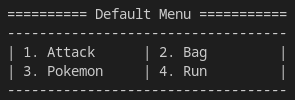
\includegraphics[height=2cm]{media/Menu.png}\end{center}
  
  \section{Unit testing and debugging}
    
\end{document}
